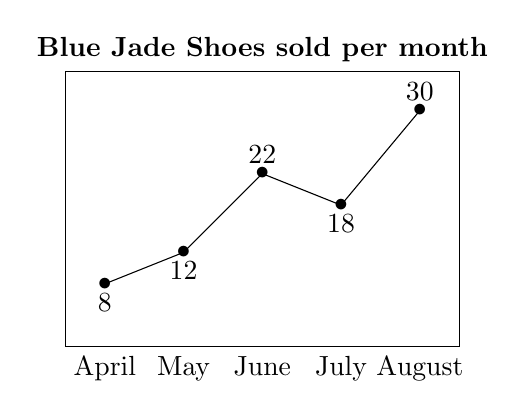
\begin{tikzpicture}
\draw (3,3.5)node[anchor=south]{\textbf{Blue Jade Shoes sold per month}};
\draw(0.5,0)rectangle(5.5,3.5)(1,0)node[anchor=north]{April}(2,0)node[anchor=north]{May}(3,0)node[anchor=north]{June}(4,0)node[anchor=north]{July}(5,0)node[anchor=north]{August};
\draw(1,.8)node{$\bullet$}node[anchor=north]{$8$}--(2,1.2)node{$\bullet$}node[anchor=north]{$12$}--(3,2.2)node{$\bullet$}node[anchor=south]{$22$}--(4,1.8)node{$\bullet$}node[anchor=north]{$18$}--(5,3)node{$\bullet$}node[anchor=south]{$30$};
\end{tikzpicture}

The line graph above shows the number of
blue jade shoes sold by Tian Jewelers
from April to August of 1961.

Tian Jewelers sold how many more shoes in
August than in April and July combined?



\ifsat
	\begin{enumerate}[label=\Alph*)]
		\item $22$
		\item $12$
		\item $4$%
		\item $2$
	\end{enumerate}
\else
\fi

\ifacteven
	\begin{enumerate}[label=\textbf{\Alph*.},itemsep=\fill,align=left]
		\setcounter{enumii}{5}
		\item $22$
		\item $12$
		\item $4$%
		\addtocounter{enumii}{1}
		\item $2$
		\item $0$
	\end{enumerate}
\else
\fi

\ifactodd
	\begin{enumerate}[label=\textbf{\Alph*.},itemsep=\fill,align=left]
		\item $22$
		\item $12$
		\item $4$%
		\item $2$
		\item $0$
	\end{enumerate}
\else
\fi

\ifgridin
 $4$%
		
\else
\fi

